\section{Implementation}
The main goal for realising client side compilation is to extend the existing virtual labs to add support to work as an online coding platform. The current implementation which can be used to compile and run code written in different languages, starting with python using pyodide.
\begin{figure}[h]
    \centering
    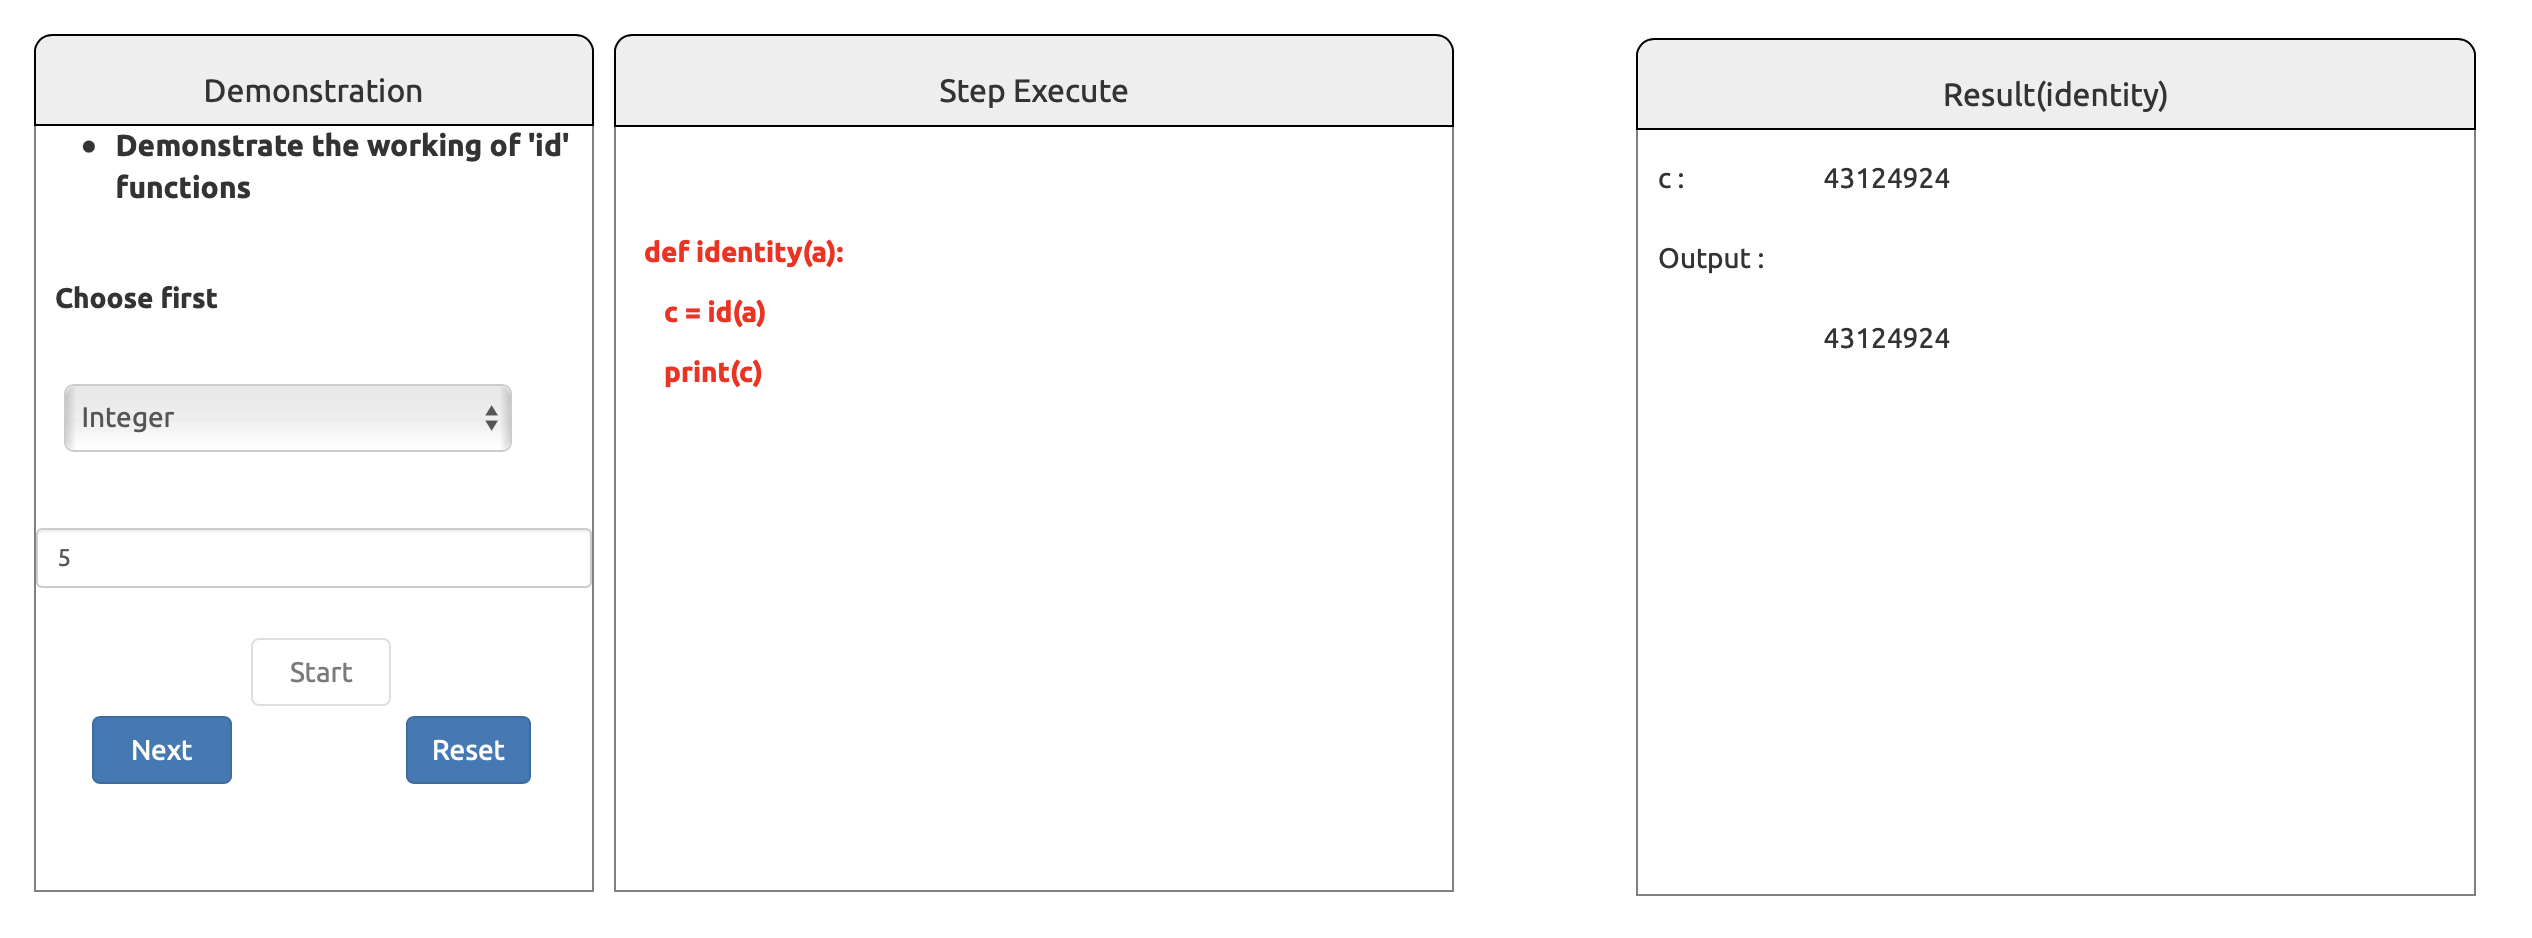
\includegraphics[width=0.8\linewidth]{images/existing-vlabs.png}
    \caption{The current implementation of virtual labs}
    \label{fig:existing-vlabs}
\end{figure}
\begin{figure}[h]
    \centering
    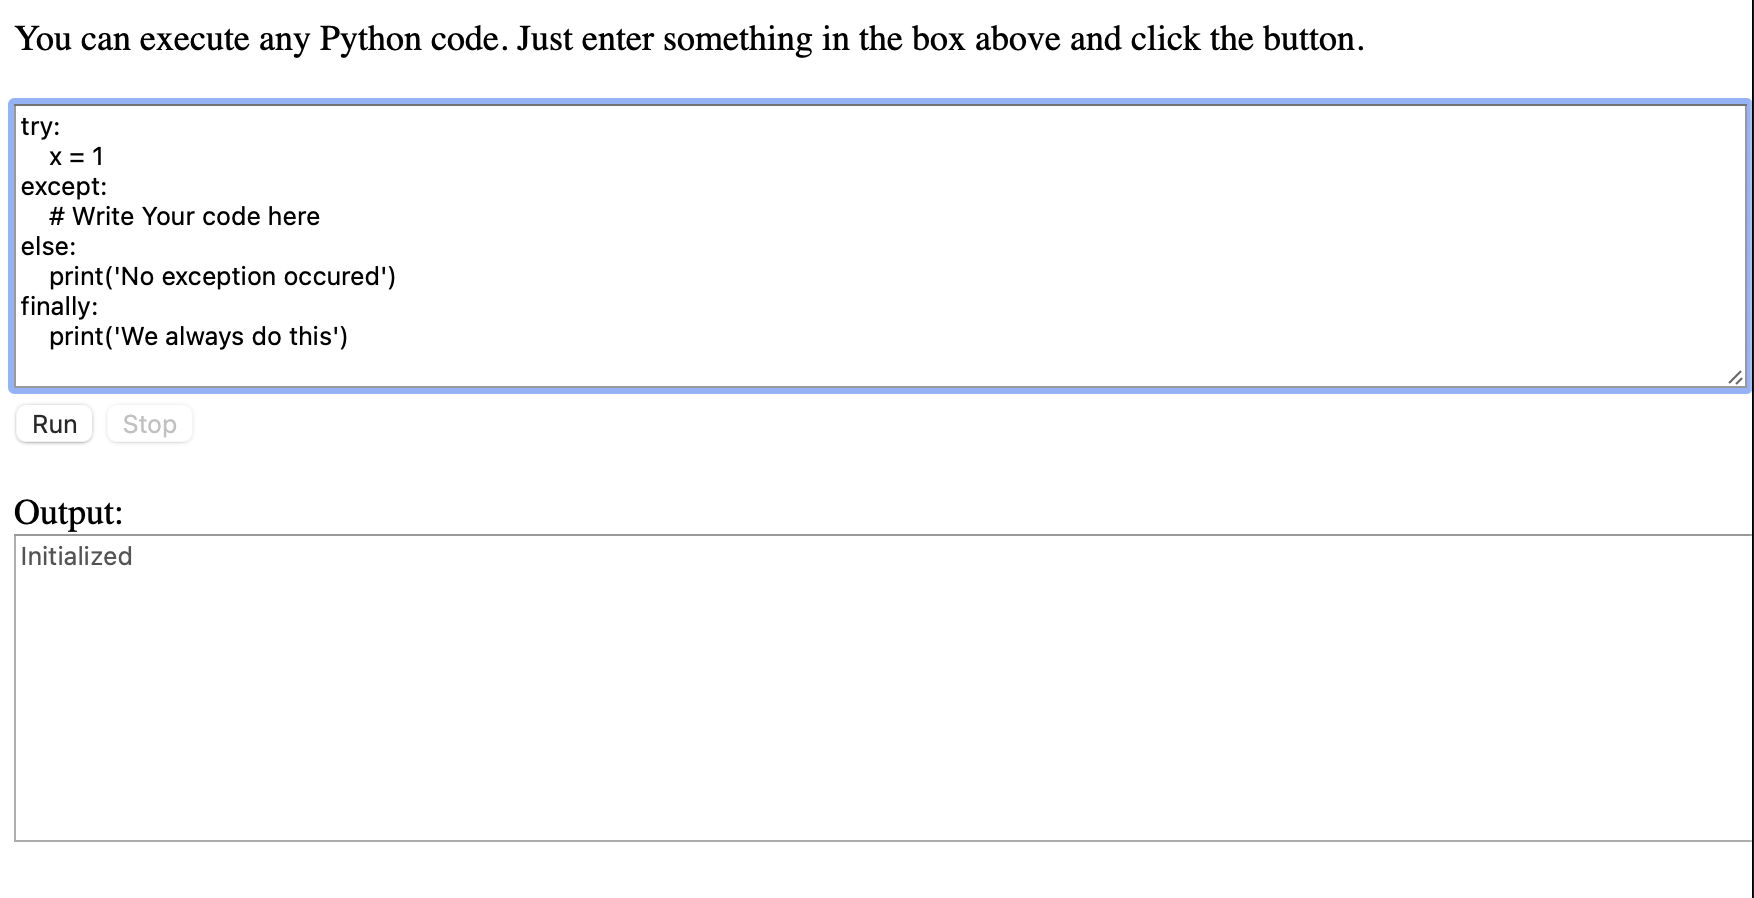
\includegraphics[width=0.8\textwidth]{images/impl-demo.png}
    \caption{Client side compiling using Pyodide}
    \label{fig:implementation}
\end{figure}
\\
For implementation, we closesly follow the documentation of Pyodide, and implement a very lightweight version of it. The screenshot of the same can be found in Fig \ref{fig:implementation}\footnote{Source code for the same can be found at \url{https://github.com/vjspranav/Pyodide-implementation}}. Considering all the requirements, we have a very basic implementation that takes care of:
\begin{itemize}
    \item Loading the python interpreter and running the code client side.
    \item Allowing a user to interrupt the execution of the code.
    \item Automatically stopping the execution of the code after a certain time limit.
    \item Disabling editing to a specific section of the code.
\end{itemize}


Intially we directly implemented using JS, and then from the bug analysis and requirement study we realised the requirement of code interrupt as discussed in 4.3. We go ahead with the implementation of the same using web workers.
The interruption is especially the focus as it can heavily influence the user's experience and can cause severe lags on the browser in cases of infinitiley running codes.
